\documentclass[a2paper, 10pt]{article}
\usepackage[a2paper]{geometry}
\usepackage[dvips]{color,graphicx}
\usepackage[dvips, bookmarks, colorlinks=false]{hyperref}
\usepackage{supertabular}
\usepackage{longtable}
\usepackage{tabularx}

%\pdfpagewidth and \pdfpageheight is only good for pdflatex
%\pdfpagewidth 13in
%\pdfpageheight 22in

\addtolength{\textheight}{5cm}
\addtolength{\textwidth}{5cm}
\addtolength{\hoffset}{-3cm}
\addtolength{\voffset}{-3cm}

%opening
\title{Report of the sequences of 2010 accessions in view of 149-snp data}
\author{Yu Huang}

\begin{document}

\maketitle

\begin{abstract}
\end{abstract}

\section{Group the 2010 accessions}

Based on the number of fragments, 248 2010 accessions are grouped into five tables. Table~\ref{tatg0} corresponds to 1 to 10 fragments. Table~\ref{tatg1} corresponds to 10 to 50 fragments. Table~\ref{tatg2} corresponds to 100 to 150 fragments. Table~\ref{tatg3} corresponds to 150 to 200 fragments. Table~\ref{tatg4} corresponds to 1300 to 1600 fragments.


\begin{table}
\caption{The number of alignments for these strains is from 1 to 1 falling into (1, 10). 1 distinct alignment combinations. alignment-type is id for one kind of distinct alignment combination. \#fragments is the number of fragments sequenced in 2010. \#149snps is the number of the 149 snps falling into that strain's fragments. Figure~\ref{fatg0} is an example chromosome chart of this table.}
\begin{tabular}{|r|r|r|r|r|r|r|r|r|r|r|r|r|r|r|}
\hline
\multicolumn{4}{|c|}{accession table} & \multicolumn{8}{|c|}{ecotype table} & \multicolumn{3}{|c|}{fragments info} \\
\hline
id & name & origin & number & id & name & nativename & stockparent & lat & lon & site & country & alignment-type & \#fragments & \#149snps\\
\hline
\multicolumn{13}{|c|}{54 strains} \\
\hline
385 & Aa-0 & None & None & 7000 & CS28007 & Aa-0 & CS6600 & 50.9167 & 9.57073 & Aa & GER & 105 & 1 & 0  \\
386 & Abd-0 & None & None & 6986 & CS28008 & Abd-0 & CS932 & 57.1539 & -2.2207 & Abd & UK & 105 & 1 & 0  \\
387 & Ak-1 & None & None & 6987 & CS28011 & Ak-1 & CS6602 & 48.0683 & 7.62551 & Ak & GER & 105 & 1 & 0  \\
388 & Ba-1 & None & None & 7014 & CS28053 & Ba-1 & CS6607 & 56.5459 & -4.79821 & Black Mount (Ba) & UK & 105 & 1 & 0  \\
389 & Bl-1 & None & None & 7025 & CS28078 & Bl-1 & CS6615 & 44.5041 & 11.3396 & Bl & ITA & 105 & 1 & 0  \\
390 & Bla-10 & None & None & 7016 & CS28085 & Bla-10 & CS6622 & 41.6833 & 2.8 & Bla & ESP & 105 & 1 & 0  \\
391 & Ca-0 & None & None & 7062 & CS28128 & Ca-0 & CS6658 & 50.2981 & 8.26607 & Ca & GER & 105 & 1 & 0  \\
392 & Cal-0 & None & None & 7061 & CS28129 & Cal-0 & CS6659 & 53.2699 & -1.64293 & Cal & UK & 105 & 1 & 0  \\
393 & Chi-0 & None & None & 7072 & CS28136 & Chi-0 & CS6664 & 53.7502 & 34.7361 & Chi & RUS & 105 & 1 & 0  \\
394 & Cnt-1 & None & None & 7064 & CS28160 & Cnt-1 & CS6921 & 51.3 & 1.1 & Canterbury (Sullivan garden) & UK & 105 & 1 & 0  \\
395 & CS6188 & None & None & 7332 & CS28728 & Seattle-0 & CS6188 & 47.0 & -122.2 & Seattle & USA & 105 & 1 & 0  \\
396 & Da-0 & None & None & 7094 & CS28200 & Da-0 & CS6676 & 49.8724 & 8.65081 & Da & GER & 105 & 1 & 0  \\
397 & Da-1-12 & None & None & 7460 & CS28201 & Da(1)-12 & CS917 & None & None & Unknown - Czech Republic & CZE & 105 & 1 & 0  \\
398 & Db-1 & None & None & 7419 & CS28203 & Db-1 & CS6678 & 50.3058 & 8.32213 & Tenne & GER & 105 & 1 & 0  \\
399 & Dig & None & None & 7096 & CS28205 & Di-G & CS910 & 47.3239 & 5.04278 & Di & FRA & 105 & 1 & 0  \\
400 & Dra-0 & None & None & 7103 & CS28212 & Dra-0 & CS6685 & 49.4167 & 16.2667 & Dra & CZE & 105 & 1 & 0  \\
401 & Ema-1 & None & None & 7109 & CS28229 & Ema-1 & CS6923 & 51.3 & 0.5 & Ema & UK & 105 & 1 & 0  \\
402 & En-2+ & None & None &  &  &  &  &  &  &  &  & 105 & 1 & 0  \\
403 & Ep-0 & None & None & 7123 & CS28236 & Ep-0 & CS6697 & 50.1721 & 8.38912 & Ep & GER & 105 & 1 & 0  \\
404 & Er-0 & None & None & 7125 & CS28239 & Er-0 & CS6698 & 49.5955 & 11.0087 & Er & GER & 105 & 1 & 0  \\
405 & Est & None & None & 7127 & CS28242 & Est & CS6173 & 58.6656 & 24.9871 & EstGER & GER & 105 & 1 & 0  \\
406 & Et-0 & None & None & 7130 & CS28246 & Et-0 & CS6702 & 44.6447 & 2.56481 & Et & FRA & 105 & 1 & 0  \\
407 & Fr-2 & None & None & 7133 & CS28266 & Fr-2 & CS6708 & 50.1102 & 8.6822 & Fr & GER & 105 & 1 & 0  \\
408 & Gie-0 & None & None & 7147 & CS28280 & Gie-0 & CS6720 & 50.584 & 8.67825 & Gie & GER & 105 & 1 & 0  \\
409 & Gre-0 & None & None & 7160 & CS28329 & Gre-0 & CS6729 & 43.178 & -85.2532 & Gre & USA & 105 & 1 & 0  \\
410 & Ha-0 & None & None & 7163 & CS28336 & Ha-0 & CS6733 & 52.3721 & 9.73569 & Ha & GER & 105 & 1 & 0  \\
411 & Hau-0 & None & None & 7164 & CS28343 & Hau-0 & CS6734 & 55.675 & 12.5686 & Hau & DEN & 105 & 1 & 0  \\
412 & Hl-3 & None & None & 7172 & CS28349 & Hl-3 & CS6904 & 52.1444 & 9.37827 & Hl & GER & 105 & 1 & 0  \\
413 & Je-0 & None & None & 7181 & CS28364 & Je-0 & CS6742 & 50.927 & 11.587 & Je & GER & 105 & 1 & 0  \\
414 & Jl-3 & None & None & 7424 & CS28369 & Jl-3 & CS6745 & 49.2 & 16.6166 & Br & CZE & 105 & 1 & 0  \\
415 & Kb-0 & None & None & 7202 & CS28380 & Kb-0 & CS6753 & 50.1797 & 8.50861 & Kb & GER & 105 & 1 & 0  \\
416 & Kend-L & None & None &  &  &  &  &  &  &  &  & 105 & 1 & 0  \\
417 & Kil-0 & None & None & 7192 & CS28386 & Kil-0 & CS6754 & 55.6395 & -5.66364 & Killean (Kil) & UK & 105 & 1 & 0  \\
418 & Li-7 & None & None & 7231 & CS28461 & Li-7 & CS6778 & 50.3833 & 8.0666 & Li & GER & 105 & 1 & 0  \\
419 & Ll-1 & None & None & 7238 & CS28471 & Ll-1 & CS6782 & 41.59 & 2.49 & Ll & ESP & 105 & 1 & 0  \\
438 & Lyrata\_Justin & None & None &  &  &  &  &  &  &  &  & 105 & 1 & 0  \\
420 & Ma-0 & None & None & 7245 & CS28488 & Ma-0 & CS6789 & 50.8167 & 8.7667 & Ma & GER & 105 & 1 & 0  \\
421 & Mh-0 & None & None & 7255 & CS28492 & Mh-0 & CS6792 & 50.95 & 7.5 & Mh & POL & 105 & 1 & 0  \\
422 & Nd-0 & None & None & 7265 & CS28528 & Nd-0 & CS6803 & 50.0 & 10.0 & Nd & SUI & 105 & 1 & 0  \\
423 & No-0 & None & None & 7275 & CS28564 & No-0 & CS3081 & 51.0581 & 13.2995 & No & GER & 105 & 1 & 0  \\
424 & Nw-4 & None & None & 7262 & CS28577 & Nw-4 & CS6815 & 50.5 & 8.5 & Nw & GER & 105 & 1 & 0  \\
425 & Ob-0 & None & None & 7276 & CS28579 & Ob-0 & CS6816 & 50.2 & 8.5833 & Ob & GER & 105 & 1 & 0  \\
426 & Or-0 & None & None & 7282 & CS28587 & Or-0 & CS6822 & 50.3827 & 8.01161 & Or & GER & 105 & 1 & 0  \\
427 & Pog-0 & None & None & 7306 & CS28650 & Pog-0 & CS6842 & 49.2655 & -123.206 & Pog & CAN & 105 & 1 & 0  \\
428 & RLD-1 & None & None & 7471 & CS28687 & RLD-1 & CS913 & None & None & UNKNOWN & UNK & 105 & 1 & 0  \\
429 & Sf-2 & None & None & 7328 & CS28731 & Sf-2 & CS6857 & 41.7833 & 3.03333 & Sf & ESP & 105 & 1 & 0  \\
430 & Ste-0 & None & None & 7346 & CS28750 & Ste-0 & CS6864 & 52.6058 & 11.8558 & Stendal & GER & 105 & 1 & 0  \\
431 & Te-0 & None & None & 7352 & CS28757 & Te-0 & CS6918 & 60.0585 & 23.2982 & Te & FIN & 105 & 1 & 0  \\
432 & Tol-0 & None & None & 7356 & CS28761 & Tol-0 & CS8020 & 41.6639 & -83.5553 & Tol & USA & 105 & 1 & 0  \\
433 & Tu-1 & None & None & 7376 & CS28784 & Tu-1 & CS6876 & 45.0 & 7.5 & Tu & ITA & 105 & 1 & 0  \\
434 & Uk-4 & None & None & 7381 & CS28790 & Uk-4 & CS6882 & 48.0333 & 7.7667 & Uk & GER & 105 & 1 & 0  \\
435 & War-0 & None & None & 7477 & CS28812 & WAR & CS8143 & 41.7302 & -71.2825 & Lincoln Woods State Park & USA & 105 & 1 & 0  \\
436 & Wt-1 & None & None & 7406 & CS28831 & Wt-1 & CS6892 & 52.3 & 9.3 & Wt & GER & 105 & 1 & 0  \\
437 & Zu-1 & None & None & 7418 & CS28847 & Zu-1 & CS6903 & 47.3667 & 8.55 & Zu & SUI & 105 & 1 & 0  \\
\hline
\end{tabular}
\label{tatg0}
\end{table}

\begin{figure}
\includegraphics[width=1\textwidth, height=1\textheight]{figures/chr_2010_alignment_type105_149snps.eps}
\caption{Red ticks are locations of 149 snps. Black blocks are locations of fragments.}\label{fatg0}
\end{figure}

\begin{table}
\caption{The number of alignments for these strains is from 38 to 38 falling into (10, 50). 1 distinct alignment combinations. alignment-type is id for one kind of distinct alignment combination. \#fragments is the number of fragments sequenced in 2010. \#149snps is the number of the 149 snps falling into that strain's fragments. Figure~\ref{fatg1} is an example chromosome chart of this table.}
\begin{tabular}{|r|r|r|r|r|r|r|r|r|r|r|r|r|r|r|}
\hline
\multicolumn{4}{|c|}{accession table} & \multicolumn{8}{|c|}{ecotype table} & \multicolumn{3}{|c|}{fragments info} \\
\hline
id & name & origin & number & id & name & nativename & stockparent & lat & lon & site & country & alignment-type & \#fragments & \#149snps\\
\hline
\multicolumn{13}{|c|}{1 strains} \\
\hline
97 & PNA-4 & None & None &  &  &  &  &  &  &  &  & 97 & 38 & 3  \\
\hline
\end{tabular}
\label{tatg1}
\end{table}

\begin{figure}
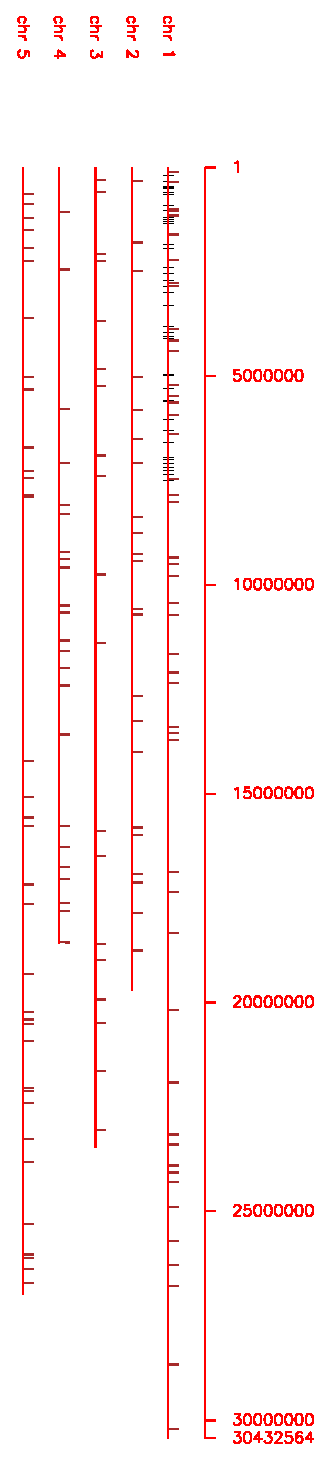
\includegraphics[width=1\textwidth, height=1\textheight]{figures/chr_2010_alignment_type97_149snps.eps}
\caption{Red ticks are locations of 149 snps. Black blocks are locations of fragments.}\label{fatg1}
\end{figure}

\begin{table}
\caption{The number of alignments for these strains is from 112 to 114 falling into (100, 150). 6 distinct alignment combinations. alignment-type is id for one kind of distinct alignment combination. \#fragments is the number of fragments sequenced in 2010. \#149snps is the number of the 149 snps falling into that strain's fragments. Figure~\ref{fatg2} is an example chromosome chart of this table.}
\begin{tabular}{|r|r|r|r|r|r|r|r|r|r|r|r|r|r|r|}
\hline
\multicolumn{4}{|c|}{accession table} & \multicolumn{8}{|c|}{ecotype table} & \multicolumn{3}{|c|}{fragments info} \\
\hline
id & name & origin & number & id & name & nativename & stockparent & lat & lon & site & country & alignment-type & \#fragments & \#149snps\\
\hline
\multicolumn{13}{|c|}{96 strains} \\
\hline
315 & Alc-0 & None & None & 8252 & Alc-0 & Alc-0 & N1656 & 40.31 & -3.22 & Alc & ESP & 99 & 113 & 3  \\
291 & Algutsrum & None & None & 8230 & Algutsrum & Algutsrum &  & 56.68 & 16.5 & Algutsrum & SWE & 99 & 113 & 3  \\
303 & Ang-0 & None & None & 8254 & Ang-0 & Ang-0 & N949 & 50.3 & 5.3 & Ang & BEL & 99 & 113 & 3  \\
355 & App-1-4 & None & None & 8255 & App1-4 & App1-4 &  & 56.3333 & 15.9667 & App1 & SWE & 99 & 113 & 3  \\
357 & B�-1-2 & None & None & 8256 & B�1-2 & B�1-2 &  & 56.4 & 12.9 & B� & SWE & 99 & 113 & 3  \\
358 & B�-3-3 & None & None & 8257 & B�3-3 & B�3-3 &  & 56.4 & 12.9 & B� & SWE & 99 & 113 & 3  \\
359 & B�-4-1 & None & None & 8258 & B�4-1 & B�4-1 &  & 56.4 & 12.9 & B� & SWE & 99 & 113 & 3  \\
360 & B�-5-1 & None & None & 8259 & B�5-1 & B�5-1 &  & 56.4 & 12.9 & B� & SWE & 99 & 113 & 3  \\
299 & Bg-2 & None & None & 8261 & Bg-2 & Bg-2 & CS22342 & 47.6479 & -122.305 & BG & USA & 99 & 113 & 3  \\
316 & Bla-1 & None & None & 8264 & Bla-1 & Bla-1 & N971 & 41.6833 & 2.8 & Bla & ESP & 99 & 113 & 3  \\
317 & Blh-1 & None & None & 8265 & Blh-1 & Blh-1 & N1031 & 48.0 & 19.0 & Blh & CZE & 99 & 113 & 3  \\
350 & Boo-2-1 & None & None & 8266 & Boo2-1 & Boo2-1 &  & 55.86 & 13.51 & Boo2 & SWE & 99 & 113 & 3  \\
354 & Br�-1-6 & None & None & 8231 & Br�1-6 & Br�1-6 &  & 56.3 & 16.0 & Br�msebro & SWE & 99 & 113 & 3  \\
318 & Bs-1 & None & None & 8270 & Bs-1 & Bs-1 & N997 & 47.5 & 7.5 & Bs & SUI & 99 & 113 & 3  \\
305 & Bu-0 & None & None & 8271 & Bu-0 & Bu-0 & N1007 & 50.5 & 9.5 & Bu & GER & 99 & 113 & 3  \\
319 & Can-0 & None & None & 8274 & Can-0 & Can-0 & N1065 & 29.2144 & -13.4811 & Can & ESP & 99 & 113 & 3  \\
320 & Cen-0 & None & None & 8275 & Cen-0 & Cen-0 & N1067 & 49.0 & 0.5 & Cen & FRA & 99 & 113 & 3  \\
321 & Co & None & None & 8278 & Co & Co & N3180 & 41.25 & -8.45 & Co & POR & 99 & 113 & 3  \\
297 & Dem-4 & None & None & 8233 & Dem-4 & Dem-4 &  & 41.1876 & -87.1923 & Dem & USA & 99 & 113 & 3  \\
352 & Di-0 & None & None & 8282 & Di-0 & Di-0 & N1107 & 47.0 & 5.0 & Di & FRA & 99 & 113 & 3  \\
361 & Dra-3-1 & None & None & 8283 & Dra3-1 & Dra3-1 &  & 55.76 & 14.12 & Dra3 & SWE & 99 & 113 & 3  \\
381 & DraII-1 & None & None & 8284 & DraII-1 & DraII-1 &  & 49.4112 & 16.2815 & DraII & CZE & 104 & 112 & 3  \\
382 & DraIII-1 & None & None & 8285 & DraIII-1 & DraIII-1 &  & 49.4112 & 16.2815 & DraIII & CZE & 104 & 112 & 3  \\
378 & Duk & None & None & 6008 & Duk & Duk &  & 49.1 & 16.2 & Duk & CZE & 104 & 112 & 3  \\
374 & Eds-1 & None & None & 6016 & Eds-1 & Eds-1 &  & 62.9 & 18.4 & Eds & SWE & 99 & 113 & 3  \\
301 & En-1 & None & None & 8290 & En-1 & En-1 & N1137 & 50.0 & 8.5 & En & GER & 99 & 113 & 3  \\
346 & Fly-2-2 & None & None & 6024 & Fly2-2 & Fly2-2 &  & 55.7509 & 13.3712 & Fly2 & SWE & 99 & 113 & 3  \\
306 & Gd-1 & None & None & 8296 & Gd-1 & Gd-1 & N1185 & 53.5 & 10.5 & Gd & GER & 100 & 114 & 3  \\
322 & Ge-0 & None & None & 8297 & Ge-0 & Ge-0 & N1187 & 46.5 & 6.08 & Ge & SUI & 100 & 114 & 3  \\
302 & Gr-1 & None & None & 8300 & Gr-1 & Gr-1 & N1199 & 47.0 & 15.5 & Graz & AUT & 100 & 114 & 3  \\
356 & Gul-1-2 & None & None & 8234 & Gul1-2 & Gul1-2 &  & 56.3 & 16.0 & Gullabo & SWE & 99 & 113 & 3  \\
323 & H55 & None & None & 8303 & H55 & H55 & N923 & 49.0 & 15.0 & Relichova & CZE & 100 & 114 & 3  \\
307 & Hi-0 & None & None & 8304 & Hi-0 & Hi-0 & N1227 & 52.0 & 5.0 & Hi & NED & 100 & 114 & 3  \\
379 & Hod & None & None & 8235 & Hod & Hod &  & 48.8 & 17.1 & Hodonin & CZE & 104 & 112 & 3  \\
383 & Hov-2-2 & None & None & 8305 & Hov2-2 & Hov2-2 &  & 56.1 & 13.74 & Hov2 & SWE & 104 & 112 & 3  \\
348 & Hov-4-1 & None & None & 8306 & Hov4-1 & Hov4-1 &  & 56.1 & 13.74 & Hovdala & SWE & 99 & 113 & 3  \\
368 & Hovdala-2 & None & None & 6039 & Hovdala-2 & Hovdala-2 &  & 56.1 & 13.74 & Hovdala & SWE & 99 & 113 & 3  \\
369 & Hovdala-6 & None & None & 8307 & Hovdala-6 & Hovdala-6 &  & 56.1 & 13.74 & Hovdala & SWE & 103 & 112 & 3  \\
308 & Hs-0 & None & None & 8310 & Hs-0 & Hs-0 & N1237 & 52.24 & 9.44 & Hannover (Hannover) & GER & 99 & 113 & 3  \\
380 & HSm & None & None & 8236 & HSm & HSm &  & 49.33 & 15.76 & Horni Smrcne & CZE & 104 & 112 & 3  \\
324 & In-0 & None & None & 8311 & In-0 & In-0 & N1239 & 47.5 & 11.5 & In & AUT & 99 & 113 & 3  \\
309 & Is-0 & None & None & 8312 & Is-0 & Is-0 & N1241 & 50.5 & 7.5 & Is & GER & 99 & 113 & 3  \\
310 & Jm-0 & None & None & 8313 & Jm-0 & Jm-0 & N1259 & 49.0 & 15.0 & Jm & CZE & 100 & 114 & 3  \\
311 & Ka-0 & None & None & 8314 & Ka-0 & Ka-0 & N1267 & 47.0 & 14.0 & Ka & AUT & 100 & 114 & 3  \\
373 & K�vlinge-1 & None & None & 8237 & K�vlinge-1 & K�vlinge-1 &  & 55.8 & 13.1 & K�vlinge & SWE & 99 & 113 & 3  \\
289 & Kent & None & None & 8238 & Kent & Kent &  & 51.15 & 0.4 & Kent & UK & 99 & 113 & 3  \\
362 & Kni-1 & None & None & 6040 & Kni-1 & Kni-1 &  & 55.66 & 13.4 & Kni1 & SWE & 99 & 113 & 3  \\
293 & K�ln & None & None & 8239 & K�ln & K�ln & CS6003 & 51.0 & 7.0 & K�ln & GER & 99 & 113 & 3  \\
372 & Kulturen-1 & None & None & 8240 & Kulturen-1 & Kulturen-1 &  & 55.705 & 13.196 & Kulturen & SWE & 99 & 113 & 3  \\
298 & Kz-13 & None & None & 8321 & Kz-13 & Kz-13 & CS22445 & 49.5 & 73.1 & KZ & KAZ & 99 & 113 & 3  \\
325 & Lc-0 & None & None & 8323 & Lc-0 & Lc-0 & N1307 & 57.0 & -4.0 & Lc & UK & 99 & 113 & 3  \\
371 & Liarum & None & None & 8241 & Liarum & Liarum &  & 55.95 & 13.85 & Liarum & SWE & 99 & 113 & 3  \\
353 & Lill�-1 & None & None & 8242 & Lill�-1 & Lill�-1 &  & 56.1512 & 15.7844 & Lill� & SWE & 99 & 113 & 3  \\
326 & Lip-0 & None & None & 8325 & Lip-0 & Lip-0 & N1337 & 50.0 & 19.3 & Lip & POL & 99 & 113 & 3  \\
365 & Lis-1 & None & None & 8326 & Lis-1 & Lis-1 &  & 56.0 & 14.7 & Lis & SWE & 99 & 113 & 3  \\
366 & Lis-2 & None & None & 8222 & Lis-2 & Lis-2 &  & 56.0 & 14.7 & Lis & SWE & 99 & 113 & 3  \\
367 & Lis-5 & None & None & 8327 & Lis-5 & Lis-5 &  & 56.0 & 14.7 & Lis & SWE & 99 & 113 & 3  \\
327 & Lm-2 & None & None & 8329 & Lm-2 & Lm-2 & N1345 & 48.0 & 0.5 & Lm & FRA & 100 & 114 & 3  \\
351 & Lom-1-1 & None & None & 6042 & Lom1-1 & Lom1-1 &  & 56.09 & 13.9 & Lom1 & SWE & 99 & 113 & 3  \\
328 & Lu-1 & None & None & 8334 & Lu-1 & Lu-1 & N1353 & 55.71 & 13.2 & Lund & SWE & 99 & 113 & 3  \\
292 & Lund & None & None & 8335 & Lund & Lund &  & 55.71 & 13.2 & Lund & SWE & 99 & 113 & 3  \\
329 & Mir-0 & None & None & 8337 & Mir-0 & Mir-0 & N1379 & 44.0 & 12.37 & Mir & ITA & 100 & 114 & 3  \\
313 & N6002 & None & None & 8243 & PHW-2 & PHW-2 & N6002 & 43.0 & 11.14 & Florence & ITA & 99 & 113 & 3  \\
304 & N6034 & None & None & 8244 & PHW-34 & PHW-34 & N6034 & 48.6103 & 2.3086 & Bretagny Sur Orge & FRA & 99 & 113 & 3  \\
314 & N6187 & None & None & 8245 & Seattle-0 & Seattle-0 & N6187 & 47.0 & -122.2 & Seattle & USA & 99 & 113 & 3  \\
330 & Na-1 & None & None & 8343 & Na-1 & Na-1 & N1385 & 47.5 & 1.5 & Na & FRA & 100 & 114 & 3  \\
294 & NC-6 & None & None & 8246 & NC-6 & NC-6 &  & 35.0 & -79.18 & NC & USA & 99 & 113 & 3  \\
331 & Nw-0 & None & None & 8348 & Nw-0 & Nw-0 & N1409 & 50.5 & 8.5 & Nw & GER & 99 & 113 & 3  \\
375 & Nyl-2 & None & None & 6064 & Nyl-2 & Nyl-2 &  & 62.96 & 18.28 & Nyl & SWE & 99 & 113 & 3  \\
364 & �r-1 & None & None & 6074 & �r-1 & �r-1 &  & 56.45 & 16.11 & �rrevet & SWE & 99 & 113 & 3  \\
332 & Ost-0 & None & None & 8351 & Ost-0 & Ost-0 & N1431 & 60.25 & 18.37 & Ost & SWE & 101 & 112 & 3  \\
333 & Pa-1 & None & None & 8353 & Pa-1 & Pa-1 & N1439 & 38.07 & 13.22 & Pa & ITA & 99 & 113 & 3  \\
334 & Per-1 & None & None & 8354 & Per-1 & Per-1 & N1445 & 58.0 & 56.3167 & Per & RUS & 99 & 113 & 3  \\
335 & Petergof & None & None & 8355 & Petergof & Petergof & N926 & 59.0 & 29.0 & Petergof & RUS & 99 & 113 & 3  \\
336 & Pi-0 & None & None & 8356 & Pi-0 & Pi-0 & N1455 & 47.04 & 10.51 & Pi & AUT & 100 & 114 & 3  \\
337 & Pla-0 & None & None & 8357 & Pla-0 & Pla-0 & N1459 & 41.5 & 2.25 & Pla & ESP & 99 & 113 & 3  \\
296 & Pu-2-8 & None & None & 8363 & Pu2-8 & Pu2-8 & CS22449 & 49.42 & 16.36 & Pu2 & CZE & 99 & 113 & 3  \\
338 & Rak-2 & None & None & 8365 & Rak-2 & Rak-2 & N1485 & 49.0 & 16.0 & Rak & CZE & 100 & 114 & 3  \\
312 & Rd-0 & None & None & 8411 & Rd-0 & Rd-0 & N1483 & 50.5 & 8.5 & Rd & GER & 100 & 114 & 3  \\
347 & Rev-1 & None & None & 8369 & Rev-1 & Rev-1 &  & 55.7 & 13.4 & Rev1 & SWE & 99 & 113 & 3  \\
290 & Rsch-4 & None & None & 8374 & Rsch-4 & Rsch-4 & CS1494 & 56.3 & 34.0 & Rsch & RUS & 99 & 113 & 3  \\
339 & Rubezhnoe-1 & None & None & 8375 & Rubezhnoe-1 & Rubezhnoe-1 & N927 & 49.0 & 38.28 & Rubezhnoe & UKR & 99 & 113 & 3  \\
349 & San-2 & None & None & 8247 & San-2 & San-2 &  & 56.07 & 13.74 & Sand�kra & SWE & 99 & 113 & 3  \\
376 & Sanna-2 & None & None & 8376 & Sanna-2 & Sanna-2 &  & 62.69 & 18.0 & San & SWE & 99 & 113 & 3  \\
340 & Santa Clara & None & None & 8377 & Santa Clara & Santa Clara & N8069 & 37.21 & -121.16 & Santa Clara & USA & 99 & 113 & 3  \\
341 & Sap-0 & None & None & 8378 & Sap-0 & Sap-0 & N1507 & 49.49 & 14.24 & Sap & CZE & 99 & 113 & 3  \\
300 & Sf-1 & None & None & 8380 & Sf-1 & Sf-1 & N6855 & 41.7833 & 3.03333 & Sf & ESP & 99 & 113 & 3  \\
377 & Sr:5 & None & None & 8386 & Sr:5 & Sr:5 &  & 58.9 & 11.2 & Sr & SWE & 104 & 112 & 3  \\
342 & St-0 & None & None & 8387 & St-0 & St-0 & N1535 & 59.0 & 18.0 & St & SWE & 100 & 114 & 3  \\
363 & Stu-1-1 & None & None & 6088 & Stu1-1 & Stu1-1 &  & 56.4 & 16.11 & Stu1 & SWE & 99 & 113 & 3  \\
343 & Stw-0 & None & None & 8388 & Stw-0 & Stw-0 & N1539 & 52.0 & 36.0 & Stw & RUS & 100 & 114 & 3  \\
344 & Ta-0 & None & None & 8389 & Ta-0 & Ta-0 & N1549 & 49.5 & 14.5 & Ta & CZE & 100 & 114 & 3  \\
370 & Tottarp-2 & None & None & 6243 & Tottarp-2 & Tottarp-2 &  & 55.95 & 13.85 & Tottarp & SWE & 99 & 113 & 3  \\
345 & Tu-0 & None & None & 8395 & Tu-0 & Tu-0 & N1567 & 45.0 & 7.5 & Tu & ITA & 102 & 112 & 3  \\
295 & Vimmerby & None & None & 8249 & Vimmerby & Vimmerby &  & 57.7 & 15.8 & Vimmerby & SWE & 99 & 113 & 3  \\
384 & Will & None & None & 8250 & Will & Will &  & 55.0 & 25.0 & Wilna & LTU & 104 & 112 & 3  \\
\hline
\end{tabular}
\label{tatg2}
\end{table}

\begin{figure}
\includegraphics[width=1\textwidth, height=1\textheight]{figures/chr_2010_alignment_type101_149snps.eps}
\caption{Red ticks are locations of 149 snps. Black blocks are locations of fragments.}\label{fatg2}
\end{figure}

\begin{table}
\caption{The number of alignments for these strains is from 197 to 197 falling into (150, 200). 1 distinct alignment combinations. alignment-type is id for one kind of distinct alignment combination. \#fragments is the number of fragments sequenced in 2010. \#149snps is the number of the 149 snps falling into that strain's fragments. Figure~\ref{fatg3} is an example chromosome chart of this table.}
\begin{tabular}{|r|r|r|r|r|r|r|r|r|r|r|r|r|r|r|}
\hline
\multicolumn{4}{|c|}{accession table} & \multicolumn{8}{|c|}{ecotype table} & \multicolumn{3}{|c|}{fragments info} \\
\hline
id & name & origin & number & id & name & nativename & stockparent & lat & lon & site & country & alignment-type & \#fragments & \#149snps\\
\hline
\multicolumn{13}{|c|}{1 strains} \\
\hline
98 & M3385S & CS6183 & None & 7453 & CS28484 & M3385S & CS6183 & 59.3324 & 18.0656 & Stockholm & SWE & 98 & 197 & 6  \\
\hline
\end{tabular}
\label{tatg3}
\end{table}

\begin{figure}
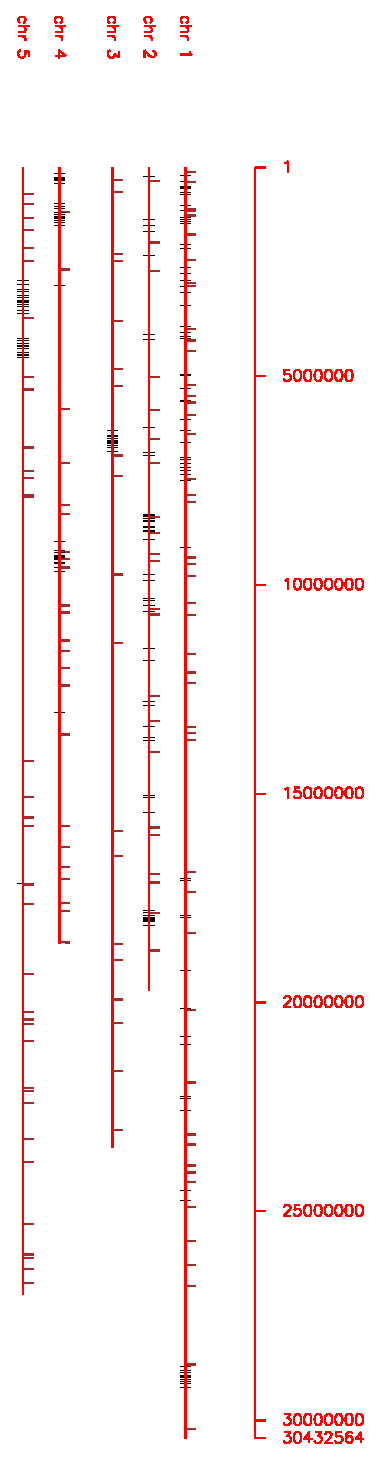
\includegraphics[width=1\textwidth, height=1\textheight]{figures/chr_2010_alignment_type98_149snps.eps}
\caption{Red ticks are locations of 149 snps. Black blocks are locations of fragments.}\label{fatg3}
\end{figure}

\begin{table}
\caption{The number of alignments for these strains is from 1330 to 1544 falling into (1300, 1600). 96 distinct alignment combinations. alignment-type is id for one kind of distinct alignment combination. \#fragments is the number of fragments sequenced in 2010. \#149snps is the number of the 149 snps falling into that strain's fragments. Figure~\ref{fatg4} is an example chromosome chart of this table.}
\begin{tabular}{|r|r|r|r|r|r|r|r|r|r|r|r|r|r|r|}
\hline
\multicolumn{4}{|c|}{accession table} & \multicolumn{8}{|c|}{ecotype table} & \multicolumn{3}{|c|}{fragments info} \\
\hline
id & name & origin & number & id & name & nativename & stockparent & lat & lon & site & country & alignment-type & \#fragments & \#149snps\\
\hline
\multicolumn{13}{|c|}{96 strains} \\
\hline
67 & Ag-0 & CS6601 & CS22630 & 8251 & Ag-0 & Ag-0 & CS22630 & 45.0 & 1.3 & Ag & FRA & 67 & 1498 & 148  \\
63 & An-1 & CS6603 & CS22626 & 8253 & An-1 & An-1 & CS22626 & 51.2167 & 4.4 & An & BEL & 63 & 1488 & 148  \\
70 & Bay-0 & CS6608 & CS22633 & 8260 & Bay-0 & Bay-0 & CS22633 & 49.0 & 11.0 & Bay & GER & 70 & 1502 & 148  \\
15 & Bil-5 &  & CS22578 & 8262 & Bil-5 & Bil-5 & CS22578 & 63.324 & 18.484 & Bil & SWE & 15 & 1507 & 148  \\
16 & Bil-7 &  & CS22579 & 8263 & Bil-7 & Bil-7 & CS22579 & 63.324 & 18.484 & Bil & SWE & 16 & 1504 & 149  \\
27 & Bor-1 &  & CS22590 & 5837 & Bor-1 & Bor-1 & CS22590 & 49.4013 & 16.2326 & Bor & CZE & 27 & 1503 & 147  \\
28 & Bor-4 &  & CS22591 & 8268 & Bor-4 & Bor-4 & CS22591 & 49.4013 & 16.2326 & Bor & CZE & 28 & 1508 & 148  \\
65 & Br-0 & CS6626 & CS22628 & 8269 & Br-0 & Br-0 & CS22628 & 49.2 & 16.6166 & Br & CZE & 65 & 1507 & 148  \\
93 & Bur-0 & CS6643 & CS22656 & 8272 & Bur-0 & Bur-0 & CS22656 & 54.1 & -6.2 & Bur & IRL & 93 & 1476 & 144  \\
57 & C24 & CS906 & CS22620 & 8273 & C24 & C24 & CS22620 & 41.25 & -8.45 & Co & POR & 57 & 1510 & 146  \\
40 & CIBC-17 &  & CS22603 & 8276 & CIBC-17 & CIBC-17 & CS22603 & 51.4083 & -0.6383 & CIBC & UK & 40 & 1518 & 148  \\
39 & CIBC-5 &  & CS22602 & 8277 & CIBC-5 & CIBC-5 & CS22602 & 51.4083 & -0.6383 & CIBC & UK & 39 & 1524 & 149  \\
62 & Col-0 & CS6673 & CS22625 & 8279 & Col-0 & Col-0 & CS22625 & 38.3 & -92.3 & Col & USA & 62 & 1544 & 149  \\
58 & CS22491 & CS22491 & CS22621 & 8429 & N13 & N13 & CS22491 & 61.36 & 34.15 & Konchezero & RUS & 58 & 1501 & 144  \\
76 & Ct-1 & CS6674 & CS22639 & 8280 & Ct-1 & Ct-1 & CS22639 & 37.3 & 15.0 & Ct & ITA & 76 & 1512 & 149  \\
51 & Cvi-0 & CS6675 & CS22614 & 8281 & Cvi-0 & Cvi-0 & CS22614 & 15.1111 & -23.6167 & Cvi & CPV & 51 & 1499 & 149  \\
9 & Eden-1 &  & CS22572 & 6009 & Eden-1 & Eden-1 & CS22572 & 62.877 & 18.177 & Eden & SWE & 9 & 1488 & 147  \\
10 & Eden-2 &  & CS22573 & 8287 & Eden-2 & Eden-2 & CS22573 & 62.877 & 18.177 & Eden & SWE & 10 & 1480 & 147  \\
94 & Edi-0 & CS6688 & CS22657 & 8288 & Edi-0 & Edi-0 & CS22657 & 56.0 & -3.0 & Edi & UK & 94 & 1484 & 147  \\
53 & Ei-2 & CS6689 & CS22616 & 8289 & Ei-2 & Ei-2 & CS22616 & 50.3 & 6.3 & Ei & GER & 53 & 1508 & 148  \\
66 & Est-1 & CS6701 & CS22629 & 8291 & Est-1 & Est-1 & CS22629 & 58.3 & 25.3 & Est & RUS & 66 & 1502 & 148  \\
13 & Fab-2 &  & CS22576 & 8292 & Fab-2 & F�b-2 & CS22576 & 63.0165 & 18.3174 & F�b & SWE & 13 & 1495 & 149  \\
14 & Fab-4 &  & CS22577 & 8293 & Fab-4 & F�b-4 & CS22577 & 63.0165 & 18.3174 & F�b & SWE & 14 & 1506 & 149  \\
82 & Fei-0 &  & CS22645 & 8294 & Fei-0 & Fei-0 & CS22645 & 40.5 & -8.32 & Fei & POR & 82 & 1495 & 147  \\
71 & Ga-0 & CS6714 & CS22634 & 8295 & Ga-0 & Ga-0 & CS22634 & 50.3 & 8.0 & Ga & GER & 71 & 1510 & 147  \\
46 & Got-22 &  & CS22609 & 8298 & Got-22 & Got-22 & CS22609 & 51.5338 & 9.9355 & G�T & GER & 46 & 1515 & 149  \\
45 & Got-7 &  & CS22608 & 8299 & Got-7 & Got-7 & CS22608 & 51.5338 & 9.9355 & G�T & GER & 45 & 1507 & 148  \\
54 & Gu-0 & CS6730 & CS22617 & 8301 & Gu-0 & Gu-0 & CS22617 & 50.3 & 8.0 & Gu & GER & 54 & 1514 & 149  \\
68 & Gy-0 & CS6732 & CS22631 & 8302 & Gy-0 & Gy-0 & CS22631 & 49.0 & 2.0 & Gy & FRA & 68 & 1512 & 148  \\
34 & HR-10 &  & CS22597 & 8308 & HR-10 & HR-10 & CS22597 & 51.4083 & -0.6383 & HR & UK & 34 & 1505 & 147  \\
33 & HR-5 &  & CS22596 & 8309 & HR-5 & HR-5 & CS22596 & 51.4083 & -0.6383 & HR & UK & 33 & 1511 & 149  \\
75 & Kas-2 & CS6751 & CS22638 & 8315 & Kas-2 & Kas-2 & CS22638 & 35.0 & 77.0 & Kas & IND & 75 & 1534 & 149  \\
91 & Kin-0 & CS6755 & CS22654 & 8316 & Kin-0 & Kin-0 & CS22654 & 44.46 & -85.37 & Kin & USA & 91 & 1486 & 146  \\
3 & Knox-10 &  & CS22566 & 8317 & Kno-10 & Kno-10 & CS22566 & 41.2816 & -86.621 & Knox & USA & 3 & 1445 & 141  \\
4 & Knox-18 &  & CS22567 & 8318 & Kno-18 & Kno-18 & CS22567 & 41.2816 & -86.621 & Knox & USA & 4 & 1474 & 144  \\
88 & Kondara & CS6175 & CS22651 & 8319 & Kondara & Kondara & CS22651 & 38.48 & 68.49 & Kondara & TJK & 88 & 1504 & 147  \\
43 & Kz-1 &  & CS22606 & 8320 & Kz-1 & Kz-1 & CS22606 & 49.5 & 73.1 & KZ & KAZ & 43 & 1504 & 149  \\
44 & Kz-9 &  & CS22607 & 8322 & Kz-9 & Kz-9 & CS22607 & 49.5 & 73.1 & KZ & KAZ & 44 & 1503 & 146  \\
55 & Ler-1 & CS6928 & CS22618 & 8324 & Ler-1 & Ler-1 & CS22618 & 47.984 & 10.8719 & Ler & GER & 55 & 1502 & 149  \\
87 & LL-0 &  & CS22650 & 8328 & LL-0 & LL-0 & CS22650 & 41.59 & 2.49 & Ll & ESP & 87 & 1511 & 148  \\
11 & Lov-1 &  & CS22574 & 6043 & L�v-1 & L�v-1 & CS22574 & 62.801 & 18.079 & L�v & SWE & 11 & 1484 & 145  \\
12 & Lov-5 &  & CS22575 & 6046 & L�v-5 & L�v-5 & CS22575 & 62.801 & 18.079 & L�v & SWE & 12 & 1497 & 148  \\
31 & Lp2-2 &  & CS22594 & 8332 & Lp2-2 & Lp2-2 & CS22594 & 49.38 & 16.81 & Lp2 & CZE & 31 & 1519 & 148  \\
32 & Lp2-6 &  & CS22595 & 8333 & Lp2-6 & Lp2-6 & CS22595 & 49.38 & 16.81 & Lp2 & CZE & 32 & 1513 & 147  \\
52 & Lz-0 & CS6788 & CS22615 & 8336 & Lz-0 & Lz-0 & CS22615 & 46.0 & 3.3 & Lz & FRA & 52 & 1515 & 146  \\
77 & Mr-0 & CS6795 & CS22640 & 8338 & Mr-0 & Mr-0 & CS22640 & 44.15 & 9.65 & Mr & ITA & 77 & 1497 & 148  \\
72 & Mrk-0 & CS6796 & CS22635 & 8339 & Mrk-0 & Mrk-0 & CS22635 & 49.0 & 9.3 & Mrk & GER & 72 & 1506 & 148  \\
92 & Ms-0 & CS6797 & CS22655 & 8340 & Ms-0 & Ms-0 & CS22655 & 55.7522 & 37.6322 & Ms & RUS & 92 & 1330 & 139  \\
79 & Mt-0 & CS6799 & CS22642 & 8341 & Mt-0 & Mt-0 & CS22642 & 32.34 & 22.46 & Mt & LIB & 79 & 1517 & 148  \\
73 & Mz-0 & CS6800 & CS22636 & 8342 & Mz-0 & Mz-0 & CS22636 & 50.3 & 8.3 & Mz & GER & 73 & 1514 & 148  \\
56 & Nd-1 & CS6922 & CS22619 & 8344 & Nd-1 & Nd-1 & CS22619 & 50.0 & 10.0 & Nd & SUI & 56 & 1505 & 147  \\
36 & NFA-10 &  & CS22599 & 8345 & NFA-10 & NFA-10 & CS22599 & 51.4083 & -0.6383 & NFA & UK & 36 & 1512 & 149  \\
35 & NFA-8 &  & CS22598 & 8346 & NFA-8 & NFA-8 & CS22598 & 51.4083 & -0.6383 & NFA & UK & 35 & 1508 & 148  \\
80 & Nok-3 & CS6810 & CS22643 & 8347 & Nok-3 & Nok-3 & CS22643 & 52.24 & 4.45 & Nok & NED & 80 & 1514 & 146  \\
21 & Omo2-1 &  & CS22584 & 8349 & �m�2-1 & �m�2-1 & CS22584 & 56.14 & 15.78 & �M�2 & SWE & 21 & 1514 & 146  \\
22 & Omo2-3 &  & CS22585 & 8350 & �m�2-3 & �m�2-3 & CS22585 & 56.14 & 15.78 & �M�2 & SWE & 22 & 1538 & 148  \\
95 & Oy-0 & CS6824 & CS22658 & 8352 & Oy-0 & Oy-0 & CS22658 & 60.23 & 6.13 & Oy & NOR & 95 & 1485 & 146  \\
8 & Pna-10 &  & CS22571 & 8358 & Pna-10 & Pna-10 & CS22571 & 42.0945 & -86.3253 & PNA & USA & 8 & 1502 & 147  \\
7 & Pna-17 &  & CS22570 & 8359 & Pna-17 & Pna-17 & CS22570 & 42.0945 & -86.3253 & PNA & USA & 7 & 1452 & 141  \\
86 & Pro-0 &  & CS22649 & 8360 & Pro-0 & Pro-0 & CS22649 & 43.25 & -6.0 & Pro & ESP & 86 & 1478 & 147  \\
30 & Pu2-23 &  & CS22593 & 8361 & Pu2-23 & Pu2-23 & CS22593 & 49.42 & 16.36 & Pu2 & CZE & 30 & 1503 & 146  \\
29 & Pu2-7 &  & CS22592 & 8362 & Pu2-7 & Pu2-7 & CS22592 & 49.42 & 16.36 & Pu2 & CZE & 29 & 1504 & 149  \\
69 & Ra-0 & CS6844 & CS22632 & 8364 & Ra-0 & Ra-0 & CS22632 & 46.0 & 3.3 & Ra & FRA & 69 & 1505 & 147  \\
47 & Ren-1 &  & CS22610 & 8367 & Ren-1 & Ren-1 & CS22610 & 48.5 & -1.41 & REN & FRA & 47 & 1519 & 146  \\
48 & Ren-11 &  & CS22611 & 8368 & Ren-11 & Ren-11 & CS22611 & 48.5 & -1.41 & REN & FRA & 48 & 1507 & 148  \\
5 & Rmx-A02 &  & CS22568 & 8370 & Rmx-A02 & Rmx-A02 & CS22568 & 42.036 & -86.511 & RMX & USA & 5 & 1449 & 144  \\
6 & Rmx-A180 &  & CS22569 & 8371 & Rmx-A180 & Rmx-A180 & CS22569 & 42.036 & -86.511 & RMX & USA & 6 & 1478 & 142  \\
2 & RRS-10 &  & CS22565 & 8372 & RRS-10 & RRS-10 & CS22565 & 41.5609 & -86.4251 & RRS & USA & 2 & 1469 & 146  \\
1 & RRS-7 &  & CS22564 & 8373 & RRS-7 & RRS-7 & CS22564 & 41.5609 & -86.4251 & RRS & USA & 1 & 1480 & 145  \\
83 & Se-0 & CS6852 & CS22646 & 8379 & Se-0 & Se-0 & CS22646 & 38.3333 & -3.53333 & Se & ESP & 83 & 1511 & 149  \\
89 & Shahdara & CS6180 & CS22652 & 8248 & Shahdara & Shahdara & CS22652 & 38.35 & 68.48 & Pamiro-Alay & TJK & 89 & 1487 & 147  \\
90 & Sorbo & CS931 & CS22653 & 8381 & Sorbo & Sorbo & CS22653 & 38.35 & 68.48 & Sorbo & TJK & 90 & 1466 & 146  \\
19 & Spr1-2 &  & CS22582 & 8382 & Spr1-2 & Spr1-2 & CS22582 & 56.3 & 16.0 & Spr1 & SWE & 19 & 1514 & 148  \\
20 & Spr1-6 &  & CS22583 & 8383 & Spr1-6 & Spr1-6 & CS22583 & 56.3 & 16.0 & Spr1 & SWE & 20 & 1497 & 148  \\
37 & Sq-1 &  & CS22600 & 8384 & Sq-1 & Sq-1 & CS22600 & 51.4083 & -0.6383 & SQ & UK & 37 & 1513 & 148  \\
38 & Sq-8 &  & CS22601 & 8385 & Sq-8 & Sq-8 & CS22601 & 51.4083 & -0.6383 & SQ & UK & 38 & 1510 & 145  \\
41 & Tamm-2 &  & CS22604 & 8390 & Tamm-2 & Tamm-2 & CS22604 & 60.0 & 23.5 & Tamm & FIN & 41 & 1509 & 148  \\
42 & Tamm-27 &  & CS22605 & 8391 & Tamm-27 & Tamm-27 & CS22605 & 60.0 & 23.5 & Tamm & FIN & 42 & 1500 & 147  \\
84 & Ts-1 & CS6868 & CS22647 & 8392 & Ts-1 & Ts-1 & CS22647 & 41.7194 & 2.93056 & Ts & ESP & 84 & 1500 & 149  \\
85 & Ts-5 & CS6871 & CS22648 & 8393 & Ts-5 & Ts-5 & CS22648 & 41.7194 & 2.93056 & Ts & ESP & 85 & 1513 & 149  \\
78 & Tsu-1 & CS6926 & CS22641 & 8394 & Tsu-1 & Tsu-1 & CS22641 & 34.43 & 136.31 & Tsu & JPN & 78 & 1499 & 149  \\
24 & Ull2-3 &  & CS22587 & 8396 & Ull2-3 & Ull2-3 & CS22587 & 56.0648 & 13.9707 & Ull2 & SWE & 24 & 1511 & 148  \\
23 & Ull2-5 &  & CS22586 & 8397 & Ull2-5 & Ull2-5 & CS22586 & 56.0648 & 13.9707 & Ull2 & SWE & 23 & 1503 & 146  \\
49 & Uod-1 &  & CS22612 & 8398 & Uod-1 & Uod-1 & CS22612 & 48.3 & 14.45 & Uod & AUT & 49 & 1507 & 147  \\
50 & Uod-7 &  & CS22613 & 8399 & Uod-7 & Uod-7 & CS22613 & 48.3 & 14.45 & Uod & AUT & 50 & 1500 & 148  \\
64 & Van-0 & CS6884 & CS22627 & 8400 & Van-0 & Van-0 & CS22627 & 49.3 & -123.0 & Van & CAN & 64 & 1497 & 149  \\
17 & Var2-1 &  & CS22580 & 8401 & V�r2-1 & V�r2-1 & CS22580 & 55.58 & 14.334 & V�r2 & SWE & 17 & 1505 & 148  \\
18 & Var2-6 &  & CS22581 & 8402 & V�r2-6 & V�r2-6 & CS22581 & 55.58 & 14.334 & V�r2 & SWE & 18 & 1513 & 148  \\
81 & Wa-1 & CS6885 & CS22644 & 8403 & Wa-1 & Wa-1 & CS22644 & 52.3 & 21.0 & Wa & POL & 81 & 1502 & 147  \\
59 & Wei-0 & CS6182 & CS22622 & 8404 & Wei-0 & Wei-0 & CS22622 & 47.25 & 8.26 & Wei & SUI & 59 & 1494 & 149  \\
60 & Ws-0 & CS6891 & CS22623 & 8405 & Ws-0 & Ws-0 & CS22623 & 52.3 & 30.0 & Ws & RUS & 60 & 1501 & 147  \\
96 & Ws-2 & CS2360 & CS22659 & 8406 & Ws-2 & Ws-2 & CS22659 & 52.3 & 30.0 & Ws & RUS & 96 & 1421 & 140  \\
74 & Wt-5 & CS6896 & CS22637 & 8407 & Wt-5 & Wt-5 & CS22637 & 52.3 & 9.3 & Wt & GER & 74 & 1504 & 146  \\
61 & Yo-0 & CS6901 & CS22624 & 8408 & Yo-0 & Yo-0 & CS22624 & 37.45 & -119.35 & Yo & USA & 61 & 1501 & 148  \\
25 & Zdr-1 &  & CS22588 & 8409 & Zdr-1 & Zdr-1 & CS22588 & 49.3853 & 16.2544 & Zdr & CZE & 25 & 1500 & 147  \\
26 & Zdr-6 &  & CS22589 & 8410 & Zdr-6 & Zdr-6 & CS22589 & 49.3853 & 16.2544 & Zdr & CZE & 26 & 1513 & 147  \\
\hline
\end{tabular}
\label{tatg4}
\end{table}

\begin{figure}
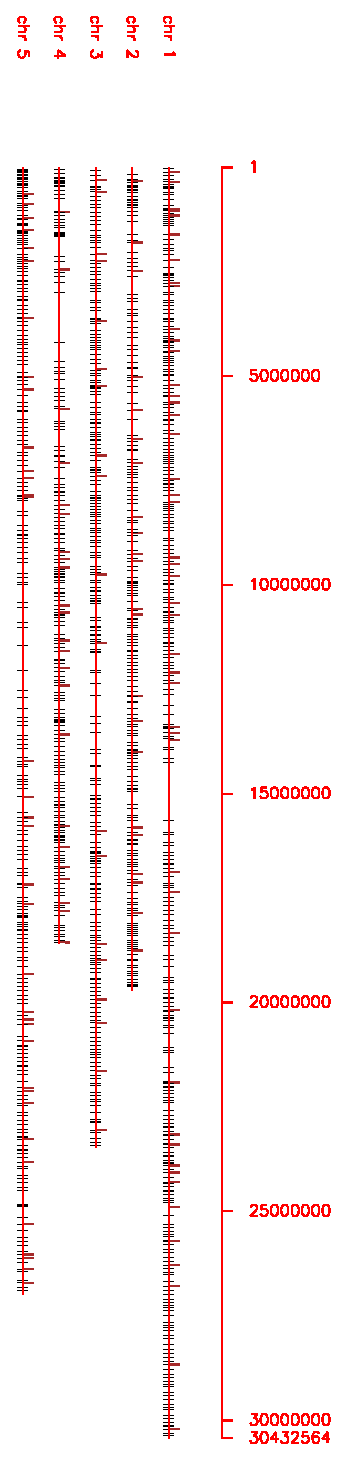
\includegraphics[width=1\textwidth, height=1\textheight]{figures/chr_2010_alignment_type92_149snps.eps}
\caption{Red ticks are locations of 149 snps. Black blocks are locations of fragments.}\label{fatg4}
\end{figure}



\end{document}
